\section{Resultados}\label{sec:resultados}

Os resultados a seguir avaliam a instanciação descrita na Seção \ref{sec:metodologia}, e não o método em si, cujas propriedades (semidefinição positiva, pseudométrica e decomposição da energia espectral) foram demonstradas nas Seções \ref{sec:tensor_rkhs} a \ref{sec:representation_geometry}. Eles são apresentados na ordem das perguntas da Subseção \ref{subsec:perguntas}, e, salvo menção explícita, os valores são os da variante de \textbf{alvo fixo}. O motivo dessa convenção fica claro com um exemplo. Na ResNet do Oxford-IIIT Pet, os $k$ vizinhos mais próximos de uma imagem na Gram conjunta de \texttt{b3} recuperam a predição do modelo em $95{,}1\%$ dos casos quando o gradiente é tomado em relação à classe predita, e em apenas $21{,}2\%$ com alvo fixo. A primeira leitura não é um acerto do método: o gradiente já carrega a predição, e reencontrá-la é como procurar uma resposta que foi escrita na pergunta. Nas imagens, as frações de execuções são frações de oito sementes, e, como discutido na Subseção \ref{subsec:estatistica}, nenhum teste pareado sobre oito sementes sobrevive à correção sobre os sete blocos de uma afirmação. Nelas, as frações devem ser lidas como contagens.

\subsection{P1: A geometria reflete o comportamento do modelo?}\label{subsec:res_comportamento}

Se o espaço reflete o entendimento do modelo, os vizinhos de uma amostra devem ter a mesma predição que ela, as amostras que o modelo erra devem estar em regiões ambíguas e as classes que o modelo confunde devem estar próximas entre si. A Tabela \ref{tab:res_estabilidade} e a Figura \ref{fig:res_estabilidade} apresentam essas leituras para as dez bases tabulares, e a Tabela \ref{tab:res_arquitetura}, para as bases de imagens.

\begin{table}[pos=htbp]
\centering
\caption{Leituras de comportamento nas dez bases tabulares (cinquenta execuções, alvo fixo). Média entre bases, do \texttt{stem} a \texttt{b6}, o piso cruzado da Gram conjunta, que é plano na profundidade, e a fração das execuções em que a Gram conjunta supera estritamente esse piso. As leituras de acerto e de erro exigem ao menos dez erros na amostra e são definidas em 31 execuções. As leituras espectrais não se aplicam à análise representacional (RSA).}
\label{tab:res_estabilidade}
\footnotesize
\setlength{\tabcolsep}{4pt}
\begin{tabular}{l c c c c c}
\hline
Leitura & Conjunta & Ativações & RSA & Piso & Acima do piso \\
\hline
$k$-vizinhos contra a predição & $0{,}880 \to 0{,}974$ & $0{,}851 \to 0{,}972$ & $0{,}850 \to 0{,}971$ & $0{,}80$ & 100\% \\
AUC da margem para o acerto & $0{,}772 \to 0{,}875$ & $0{,}798 \to 0{,}885$ & $0{,}746 \to 0{,}853$ & $0{,}73$ & 84\% a 100\% \\
Confusão suave (Spearman) & $0{,}441 \to 0{,}391$ & $0{,}457 \to 0{,}452$ & $0{,}356 \to 0{,}342$ & $0{,}42$ & 47\% a 76\% \\
Contenção em $V_r$ ($r = Q-1$) & $0{,}561 \to 0{,}827$ & $0{,}474 \to 0{,}820$ & & $0{,}41$ & 98\% a 100\% \\
$\widehat{E}_{\mathrm{ratio}}$ para o erro & $0{,}664 \to 0{,}799$ & $0{,}659 \to 0{,}795$ & & $0{,}62$ & 81\% a 100\% \\
\hline
\end{tabular}
\end{table}

\begin{figure}[pos=htbp]
    \centering
    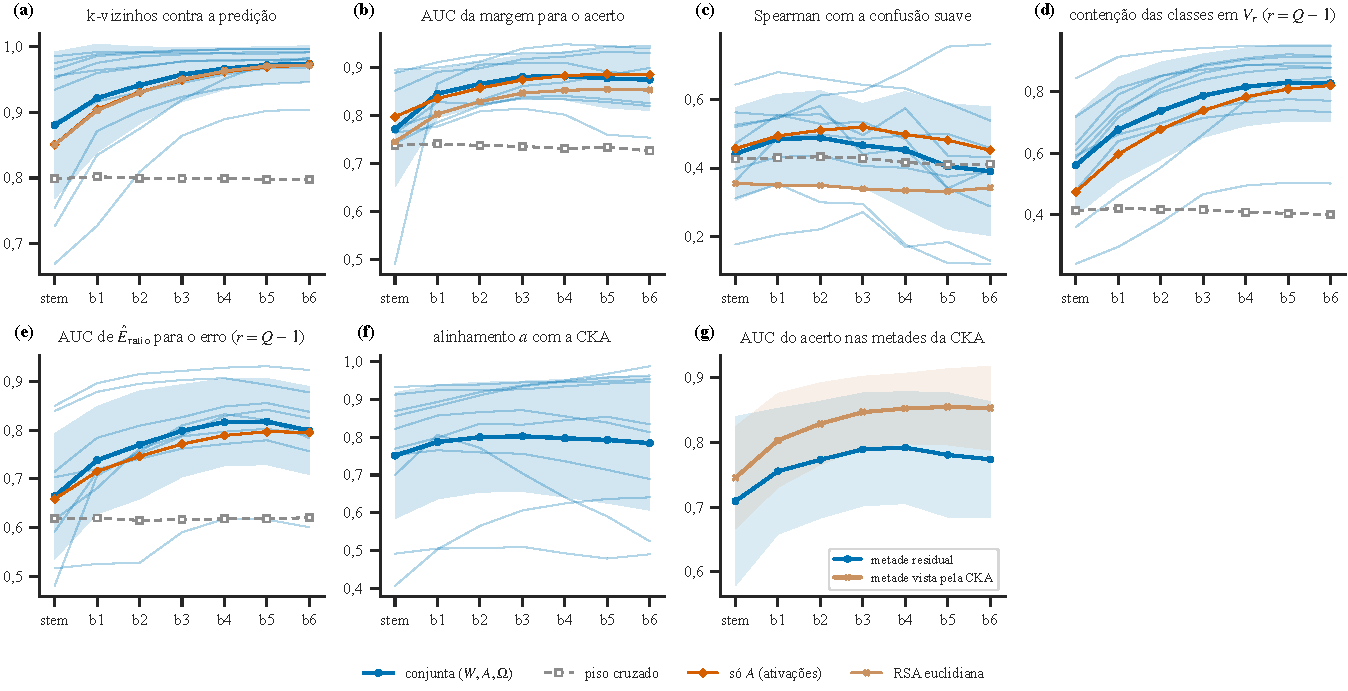
\includegraphics[width=\textwidth]{res_estabilidade.pdf}
    \caption{Leituras por bloco nas dez bases tabulares, com alvo fixo. A linha grossa é a média entre bases da Gram conjunta, as linhas finas são as bases isoladas e a faixa é o desvio entre bases. A linha tracejada é o piso cruzado, e as demais séries são a fonte de ativações isolada e a análise representacional euclidiana. (a) Recuperação da predição por $k$-vizinhos. (b) Área sob a curva ROC da margem geométrica para o acerto. (c) Concordância com a confusão suave. (d) Contenção das direções de classe em $V_r$. (e) $\widehat{E}_{\mathrm{ratio}}$ como preditor do erro. (f) Alinhamento com a Gram das ativações. (g) Acerto previsto pelas duas partes da decomposição contra a CKA.}
    \label{fig:res_estabilidade}
\end{figure}

A recuperação da predição por $k$-vizinhos fica acima do piso em todas as execuções e em todos os blocos (Figura \ref{fig:res_estabilidade}a), e a diferença é significativa em todos os blocos ($p < 0{,}05$, Wilcoxon sobre as dez bases com correção de Holm). Duas ressalvas, entretanto, limitam o que essa leitura demonstra. A primeira é que o piso é alto ($0{,}80$), e isso é uma propriedade dos dados: as classes dessas bases já são quase separáveis nos atributos brutos, e um modelo na inicialização preserva boa parte dessa estrutura. A segunda é que, nos blocos profundos, a Gram conjunta ($0{,}974$), a fonte de ativações isolada ($0{,}972$) e a RSA ($0{,}971$) praticamente coincidem, e os $k$-vizinhos nos próprios \textit{logits} chegam a $0{,}988$: ali, vizinhos em qualquer representação final recuperam a predição quase por construção. Por esse motivo, as bases de imagens funcionam como contraprova. Com 37 raças no Pet e 100 classes no CIFAR-100, o piso cai para cerca de $0{,}07$, e a Gram conjunta cresce de $0{,}095$ para $0{,}619$ na ResNet do Pet e de $0{,}060$ para $0{,}701$ no CIFAR-100, acima do piso em todas as sementes a partir de \texttt{b1} (Figuras \ref{fig:res_pets}a e \ref{fig:res_cifar}a).

A segunda leitura é a margem geométrica da Equação \eqref{eq:margem_geometrica}, isto é, o quanto um objeto está mais próximo dos objetos com a sua própria predição do que dos objetos com a predição vizinha, calculada sem acesso ao rótulo do objeto. Ela prevê se o modelo acerta, com área sob a curva de $0{,}87$ a $0{,}88$ nos blocos intermediários das bases tabulares, contra um piso de $0{,}73$, e acima do piso em todas as sementes a partir de \texttt{b1} nas três redes de imagem (Tabela \ref{tab:res_arquitetura}). A intuição é a mesma do \textit{trust score} \citep{Jiang2018} e dos $k$-vizinhos profundos \citep{Papernot2018}: uma predição cercada de vizinhos classificados de outra forma merece menos confiança. A Tabela \ref{tab:res_confianca}, entretanto, mostra que essa leitura não supera sinais de confiança que não usam o método. Nas bases tabulares, ela empata com a probabilidade máxima do \textit{softmax} ($0{,}870$) e fica abaixo da margem entre os \textit{logits} e do \textit{trust score}. Nas imagens, a margem no último bloco empata com o \textit{softmax} na ResNet do Pet ($0{,}829$) e fica abaixo dele no transformador e no CIFAR-100, e a margem nos blocos intermediários, em que a composição mais acrescenta às ativações (P2), é bem inferior. A previsão do acerto é, portanto, uma propriedade da geometria, mas não uma vantagem prática sobre sinais baratos de confiança.

\begin{table}[pos=htbp]
\centering
\caption{Previsão do acerto (área sob a curva ROC, média entre execuções): a margem geométrica da Gram conjunta, em \texttt{b3} e no último bloco, contra sinais de confiança que não usam o método. O \textit{trust score} e a distância de Mahalanobis são calculados nas ativações do último bloco, com as classes do treino.}
\label{tab:res_confianca}
\footnotesize
\setlength{\tabcolsep}{4pt}
\begin{tabular}{l c c c c c c}
\hline
 & \multicolumn{2}{c}{Margem geométrica} & \textit{Softmax} & Margem dos & \textit{Trust} & Mahalanobis \\
 & \texttt{b3} & \texttt{b6} & máximo & \textit{logits} & \textit{score} & \\
\hline
Bases tabulares & $0{,}870$ & $0{,}861$ & $0{,}870$ & $0{,}885$ & $\mathbf{0{,}930}$ & $0{,}805$ \\
Pet, ResNet & $0{,}660$ & $0{,}829$ & $0{,}829$ & $0{,}822$ & $\mathbf{0{,}848}$ & $0{,}625$ \\
Pet, transformador & $0{,}694$ & $0{,}705$ & $\mathbf{0{,}748}$ & $0{,}716$ & $0{,}722$ & $0{,}668$ \\
CIFAR-100, ResNet & $0{,}609$ & $0{,}804$ & $\mathbf{0{,}864}$ & $0{,}860$ & $0{,}827$ & $0{,}568$ \\
\hline
\end{tabular}
\end{table}

A terceira leitura, a concordância com a confusão, separa as duas famílias de dados. Nas bases tabulares, ela não se sustenta nos blocos profundos, ficando acima do piso em apenas 47\% a 49\% das execuções em \texttt{b5} e \texttt{b6} (Figura \ref{fig:res_estabilidade}c). Nas imagens, ela cresce com a profundidade, de $0{,}150$ para $0{,}662$ na ResNet do Pet e de $0{,}260$ para $0{,}670$ no CIFAR-100, contra pisos em torno de $0{,}20$, e supera o piso em todas as sementes a partir de \texttt{b1}. A diferença é simples: nas bases tabulares o modelo quase não erra, e a confusão entre a maior parte dos pares de classes é praticamente nula. Nas imagens, classes confundíveis produzem uma estrutura de confusão rica, e a geometria a reproduz.

\begin{figure}[pos=htbp]
    \centering
    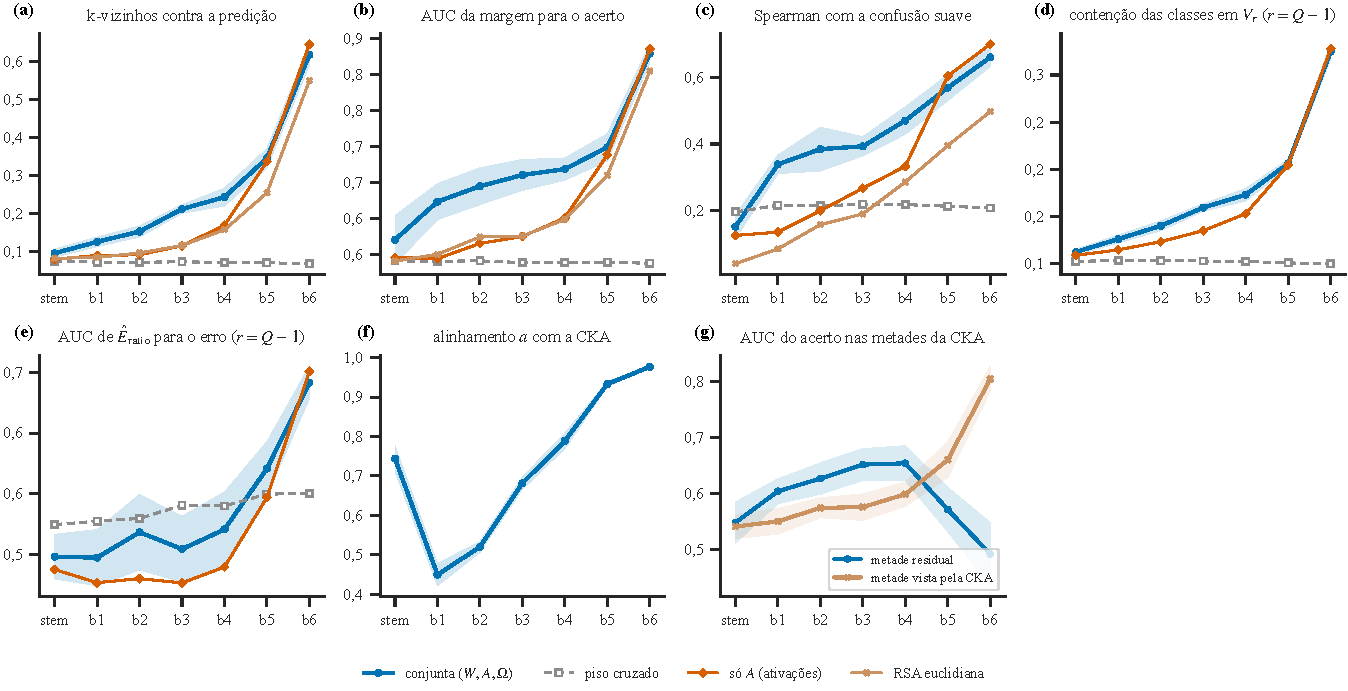
\includegraphics[width=\textwidth]{res_pets.pdf}
    \caption{As mesmas leituras da Figura \ref{fig:res_estabilidade} no Oxford-IIIT Pet, com a ResNet (oito sementes, alvo fixo). A faixa é o desvio entre sementes. Diferentemente das bases tabulares, o piso do $k$-vizinhos fica próximo do acaso ($1/37$), e a concordância com a confusão supera o piso a partir de \texttt{b1}.}
    \label{fig:res_pets}
\end{figure}

\begin{figure}[pos=htbp]
    \centering
    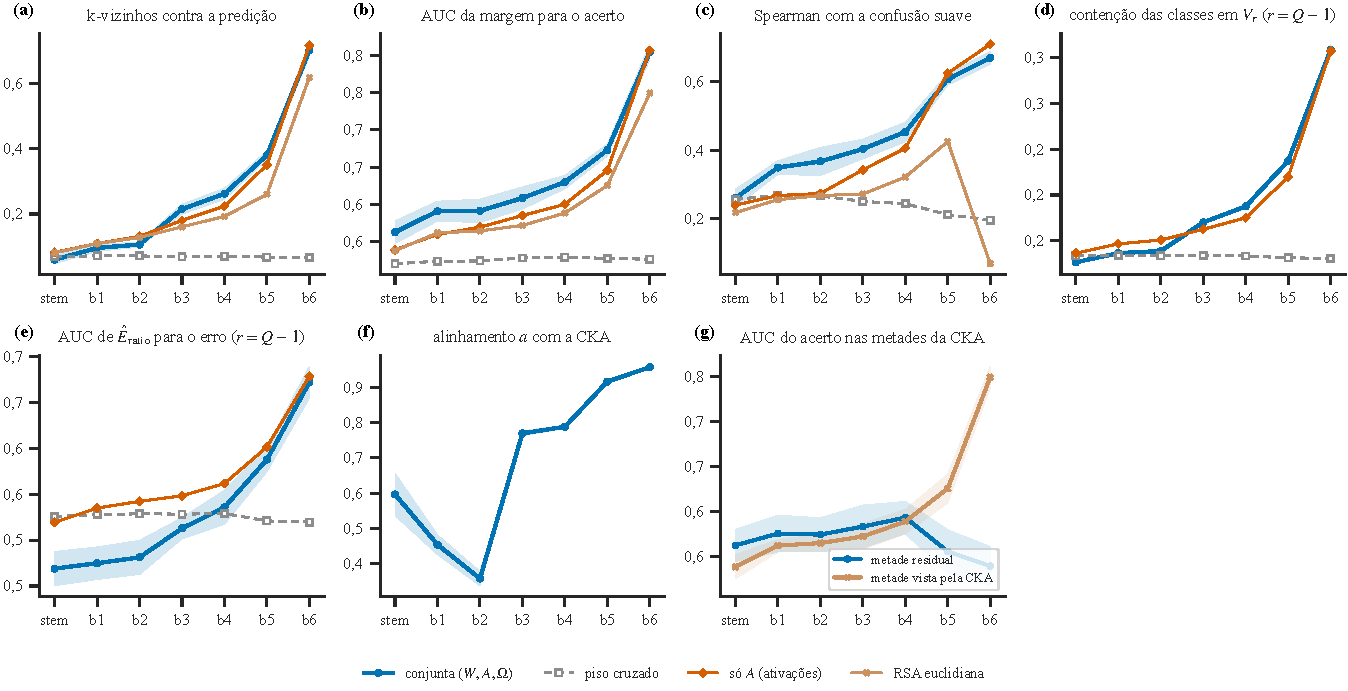
\includegraphics[width=\textwidth]{res_cifar.pdf}
    \caption{As mesmas leituras da Figura \ref{fig:res_estabilidade} no CIFAR-100, com a ResNet (oito sementes, alvo fixo, $n = 1\,000$ objetos). A faixa é o desvio entre sementes.}
    \label{fig:res_cifar}
\end{figure}

A resposta a P1 é, portanto, afirmativa para a decisão e para o erro, condicionada para a confusão, que só se sustenta quando o modelo confunde classes de forma estruturada, e negativa quanto a uma vantagem prática: a geometria reflete o comportamento, mas não o antecipa melhor do que o próprio modelo já informa nos seus \textit{logits}.

\subsection{P2: A composição acrescenta algo às fontes isoladas?}\label{subsec:res_composicao}

A pergunta tem duas partes: se a Gram conjunta supera a melhor fonte isolada e, quando supera, se isso se deve à forma multiplicativa da composição.

Contra as ativações, a resposta depende de onde a leitura é feita. Nas bases tabulares, a Gram conjunta supera a fonte de ativações na recuperação da predição em 84\% das execuções no \texttt{stem}, mas essa vantagem decresce até 32\% em \texttt{b6}, e nunca supera as ativações na concordância com a confusão. Nas redes convolucionais o padrão é o mesmo e mais nítido: na ResNet do Pet, a conjunta supera as ativações em todas as sementes de \texttt{b2} a \texttt{b4} nas três leituras de comportamento, e no CIFAR-100, na previsão do acerto, em sete ou oito das oito sementes de \texttt{b1} a \texttt{b5}. Nos dois casos a vantagem desaparece no último bloco (Figuras \ref{fig:res_pets} e \ref{fig:res_cifar}). No transformador, a conjunta só supera as ativações de forma consistente no \texttt{stem}.

Contra o gradiente isolado, a resposta é menos favorável. Na ResNet do Pet, $\Omega$ sozinho prevê o acerto tão bem quanto a composição, e melhor em \texttt{b3} e \texttt{b4} (em seis e em oito das oito sementes). A vantagem da conjunta sobre as ativações vem, portanto, de acrescentar o gradiente, e não de compor as três fontes. No CIFAR-100 e no transformador, por outro lado, a conjunta supera $\Omega$ na recuperação da predição em todas as sementes e na previsão do acerto na maioria delas, e nas bases tabulares supera $\Omega$ na concordância com a confusão em todos os blocos ($p < 0{,}05$). A fonte de parâmetros ativados, por fim, é quase redundante com as ativações, o que é esperado: a sua Gram é a forma bilinear $A_i^\top(WW^\top)A_j$, e as distâncias das duas fontes têm correlação de Spearman entre $0{,}88$ e $0{,}97$.

\begin{figure}[pos=htbp]
    \centering
    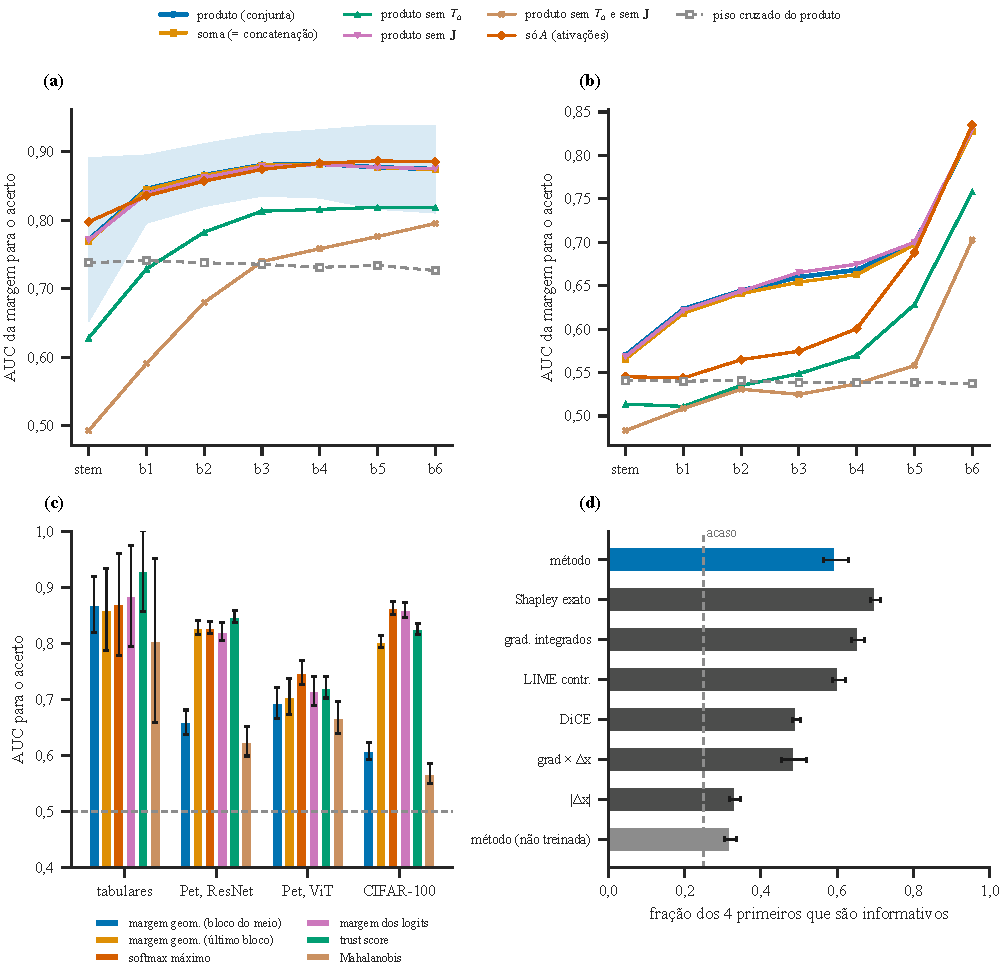
\includegraphics[width=\textwidth]{res_ablacoes.pdf}
    \caption{Ablações. (a) Área sob a curva da margem geométrica para o acerto, por bloco, nas dez bases tabulares (média entre bases, com a faixa indicando o desvio entre bases da conjunta), para o produto de Hadamard, a composição aditiva (igual à Gram da concatenação), o produto sem $T_a$, sem $\mathbf{J}$ e sem os dois, a fonte de ativações isolada e o piso cruzado do produto. (b) O mesmo na ResNet do Oxford-IIIT Pet. (c) Previsão do acerto pela margem geométrica e por sinais de confiança que não usam o método (Tabela \ref{tab:res_confianca}). (d) Dados sintéticos com quatro atributos informativos entre dezesseis: fração dos quatro primeiros atributos de cada ranking que são informativos, com o acaso tracejado (P6).}
    \label{fig:res_ablacoes}
\end{figure}

A segunda parte é respondida pelas ablações da Figura \ref{fig:res_ablacoes}. O produto de Hadamard e a composição aditiva, com as mesmas fontes e a mesma normalização, produzem praticamente os mesmos valores em todas as bases e arquiteturas: $0{,}881$ contra $0{,}881$ em \texttt{b3} nas bases tabulares, $0{,}660$ contra $0{,}654$ na ResNet do Pet, $0{,}694$ contra $0{,}694$ no transformador e $0{,}609$ contra $0{,}604$ no CIFAR-100. A forma multiplicativa, portanto, não é responsável pelo que a composição acrescenta, e uma combinação aditiva, ou a Gram da concatenação das fontes normalizadas, produziria as mesmas leituras. As duas escolhas feitas antes da composição se comportam de forma oposta. Sem a transformação angular $T_a$, todas as leituras caem, de $0{,}881$ para $0{,}813$ nas bases tabulares e de $0{,}609$ para $0{,}512$ no CIFAR-100, e o produto com $T_a$ supera o produto sem ela em 84\% a 100\% das execuções em todos os blocos e famílias, com a única exceção do último bloco do transformador. A normalização que impede uma fonte de dominar as demais é, assim, a escolha decisiva. Sem o deslocamento por $\mathbf{J}$, ao contrário, as leituras são praticamente as mesmas, de modo que o deslocamento é uma salvaguarda numérica, e não uma fonte de informação.

\subsection{P3: O método se distingue de uma simples CKA?}\label{subsec:res_cka}

A decomposição $\hat{\mathbf{G}} = a\,\hat{K}_{\mathrm{ativ}} + R$ responde a essa pergunta em termos de conteúdo. Um resultado torna a decomposição fácil de interpretar: a parte vista pela CKA, $a\,\hat{K}_{\mathrm{ativ}}$, produz exatamente os mesmos valores que a RSA euclidiana em todas as leituras, sementes e arquiteturas. Isso não é coincidência, visto que as distâncias induzidas pela Gram linear centrada das ativações são as distâncias euclidianas entre elas. A parte que a CKA enxerga é, portanto, a geometria euclidiana das ativações, e o resíduo $R$ é tudo aquilo que uma análise das ativações não enxerga.

Nas bases tabulares, o alinhamento $a$ fica entre $0{,}75$ e $0{,}80$, e o resíduo prevê o acerto pior do que a parte vista em 61\% a 77\% das execuções (Figura \ref{fig:res_estabilidade}g), o que favorece a CKA. Nas redes convolucionais, o resultado se inverte nos blocos rasos e intermediários. Na ResNet do Pet, o alinhamento cai para $0{,}45$ em \texttt{b1}, e o resíduo prevê o acerto melhor do que a parte vista em sete ou oito das oito sementes de \texttt{b1} a \texttt{b4}, invertendo-se nos dois últimos blocos, em que o alinhamento sobe para $0{,}93$ e $0{,}98$. No CIFAR-100, o alinhamento cai para $0{,}36$ em \texttt{b2}, e o resíduo vence em metade a três quartos das sementes até \texttt{b4}. No transformador, cujo alinhamento fica acima de $0{,}82$ em todos os blocos, o resíduo só vence no \texttt{stem}. A resposta a P3 é, portanto, condicionada da mesma forma que P2: o método vê algo além da CKA onde o gradiente ainda carrega informação que as ativações não têm. Esse resultado é coerente com as limitações da CKA apontadas pela literatura, que mostram que ela é dominada pelos modos de maior variância das ativações \citep{Davari2023, Klabunde2025}.

\subsection{P4: A energia espectral descreve como o modelo representa cada amostra?}\label{subsec:res_espectro}

As leituras espectrais decompõem a Gram em modos e perguntam quais direções concentram a estrutura do espaço e quanto de cada amostra vive fora delas. A primeira afirmação, de que as direções de classe estão contidas em $V_r$, é a mais robusta da instanciação. Com $r = Q-1$, ela supera o piso em todas as execuções tabulares a partir de \texttt{b1} e é significativa em todos os blocos, e a Gram conjunta supera as ativações em 78\% a 100\% das execuções em toda a profundidade (Figura \ref{fig:res_estabilidade}d). Nas imagens, os valores são menores, mas superam o piso em todas as sementes: de $0{,}112$ para $0{,}325$ na ResNet do Pet e de $0{,}137$ para $0{,}246$ no transformador, contra pisos em torno de $0{,}10$, e de $0{,}127$ para $0{,}358$ no CIFAR-100 a partir de \texttt{b2}, contra $0{,}13$. Isto é, as poucas direções dominantes do espaço construído são as direções em que o modelo separa as suas decisões.

A segunda afirmação depende da base. Nas bases tabulares, $\widehat{E}_{\mathrm{ratio}}$ prevê o erro acima do piso em 81\% a 100\% das execuções (Figura \ref{fig:res_estabilidade}e). Nas redes convolucionais, por outro lado, ela fica abaixo do piso nos blocos rasos e intermediários e só o supera no último bloco da ResNet do Pet e a partir de \texttt{b5} no CIFAR-100. No transformador, supera o piso em todas as sementes a partir de \texttt{b2}. A ideia é a mesma da detecção de amostras fora da distribuição pelo resíduo do subespaço principal \citep{Wang2022ViM}, e o resultado mostra que esse indício só é confiável onde $V_r$ já é o subespaço da decisão. A razão de energia ortogonal é, portanto, a leitura menos robusta da instanciação.

\subsection{P5: Que informação espacial sobre as representações do modelo oferecem o campo de energia e os conjuntos de nível?}\label{subsec:res_campo}

Esta subseção toma como objetos as posições espaciais de uma única imagem, conforme o Comentário \ref{rem:diagnostic}. Em cada bloco, a posição $s$ carrega as três fontes, e as matrizes de Gram de ordem $P = HW$ são compostas pelo produto de Hadamard sem a normalização angular, que fixaria a energia de todas as posições. O campo de energia é a energia retida $\widehat{E}_{s,\parallel}$ da Equação \eqref{eq:empirical_energies}, calculada sobre 111 imagens de teste da ResNet do Pet. A utilidade dessa leitura é auditar \textit{onde} o modelo representa o objeto, visto que um modelo pode acertar apoiando-se no fundo ou em um artefato da coleta \citep{Geirhos2020}.

\begin{figure}[pos=htbp]
    \centering
    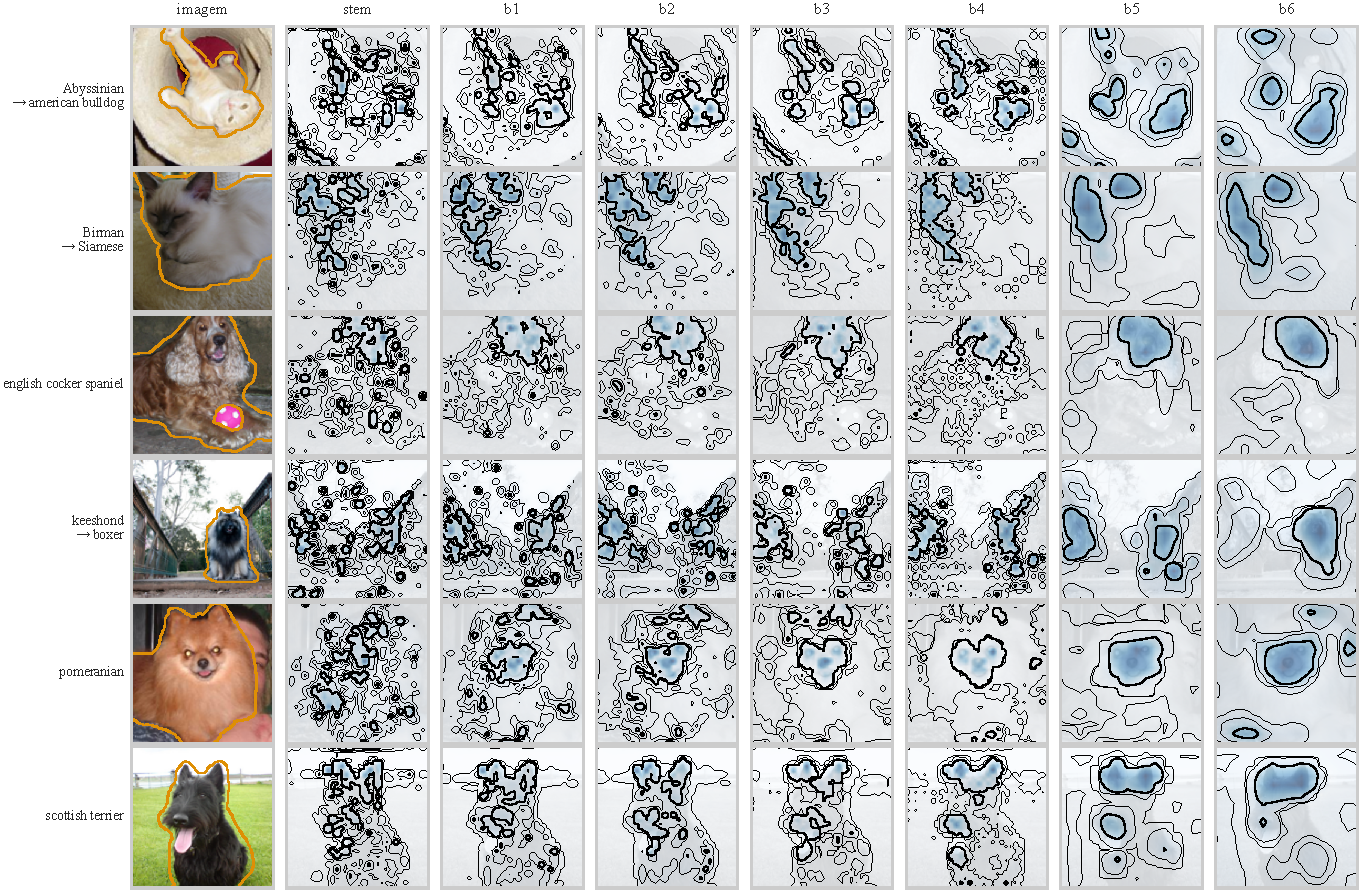
\includegraphics[width=\textwidth]{res_campo_resnet.pdf}
    \caption{Campo de energia da Gram conjunta da ResNet sobre seis imagens de teste do Oxford-IIIT Pet, do \texttt{stem} a \texttt{b6}. O contorno na primeira coluna é a máscara do animal, utilizada apenas na avaliação, e os rótulos indicam a raça verdadeira e, quando o modelo erra, a predita. Tons escuros indicam maior energia retida.}
    \label{fig:res_campo_resnet}
\end{figure}

A primeira parte da pergunta é respondida afirmativamente. Na ResNet, o campo concentra de $0{,}80$ a $0{,}89$ da sua energia sobre o animal, contra $0{,}50$ de acaso, $0{,}66$ de um mapa que marca apenas o centro, $0{,}52$ a $0{,}75$ do Grad-CAM \citep{Selvaraju2017} e $0{,}47$ a $0{,}49$ da rede não treinada. Nos blocos rasos, o campo se espalha sobre o contorno e a textura do animal, e nos profundos se concentra em poucas regiões, tipicamente a cabeça (Figura \ref{fig:res_campo_resnet}). O campo também passa na verificação por aleatorização dos pesos \citep{Adebayo2018}, com correlação entre os campos da rede treinada e da não treinada entre $-0{,}11$ e $0{,}04$. A localização, entretanto, vem principalmente do gradiente: o campo de $\Omega$ isolado concentra de $0{,}60$ a $0{,}78$ da energia sobre o animal, enquanto o das ativações isoladas fica entre $0{,}53$ e $0{,}68$.

A segunda parte examina a relação entre a ordenação espacial e a evidência da decisão. No teste de deleção \citep{Samek2017, Tomsett2020}, a ordenação pela Gram conjunta produz diferenças de área de $0{,}39$ a $0{,}50$ do \texttt{stem} a \texttt{b5}, contra $0{,}31$ do centro. A partir de \texttt{b4}, a ordenação do Grad-CAM, calculado sobre o mesmo estado e gradiente, produz uma queda maior da margem ($0{,}66$ a $0{,}79$). Esse resultado descreve o comportamento dos mapas nesse teste específico, que mede sensibilidade da decisão, e não localização. O campo do Fannar caracteriza a distribuição espacial da representação, enquanto o Grad-CAM destaca regiões sensíveis à decisão. A diferença, portanto, não estabelece a superioridade geral de um mapa sobre o outro, mas mostra que eles oferecem informações distintas \citep{Hooker2019, Nauta2023}.

\begin{figure}[pos=htbp]
    \centering
    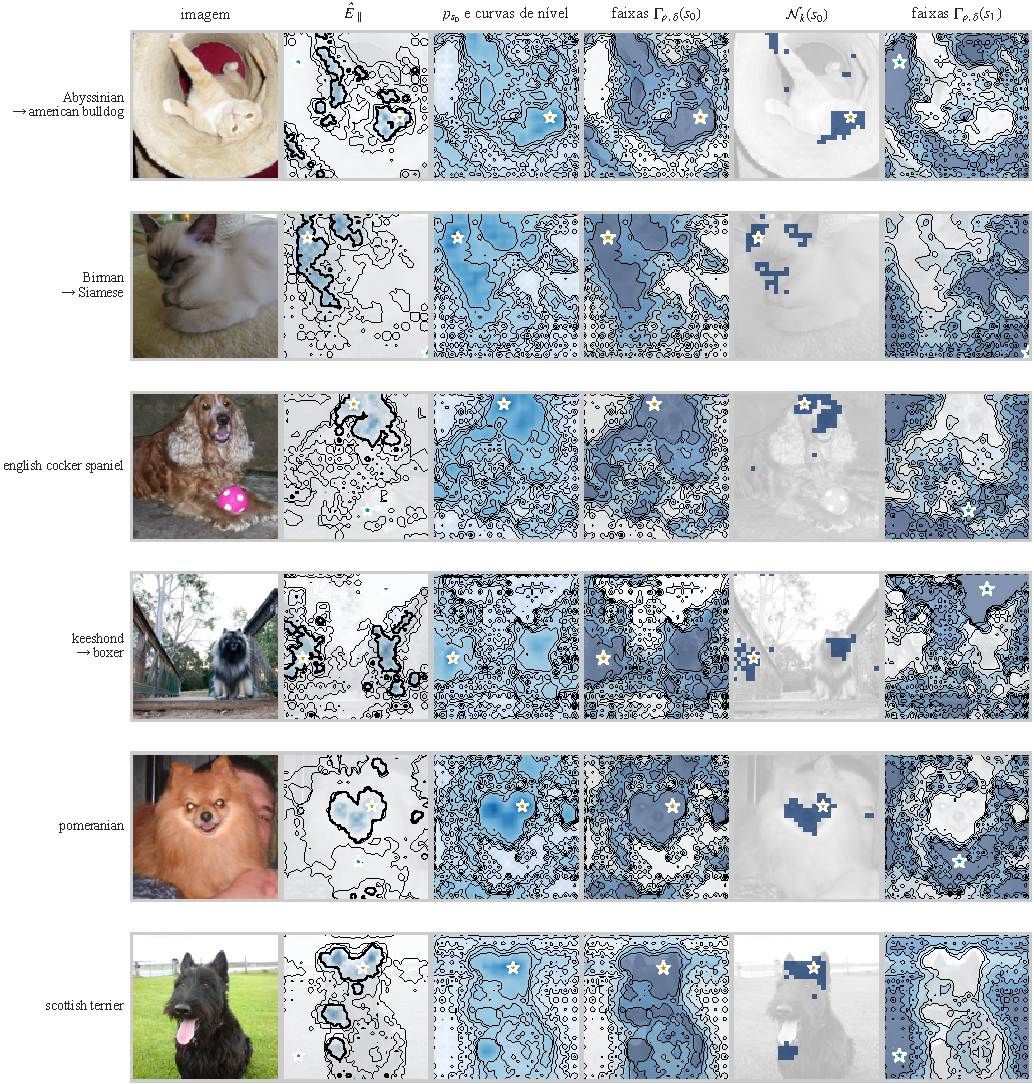
\includegraphics[width=\textwidth]{res_niveis.pdf}
    \caption{Conjuntos de nível no bloco \texttt{b4} da ResNet. Da esquerda para a direita, a figura mostra a imagem, o campo de energia com a referência $s_0$ (medoide das posições de maior energia) e $s_1$ (medoide da metade de menor energia), a função distância $p_{s_0}$ com as suas curvas de nível, as faixas de nível $\Gamma_{\rho,\delta}(s_0)$, a vizinhança $\mathcal{N}_k(s_0)$ e as faixas em torno de $s_1$.}
    \label{fig:res_niveis}
\end{figure}

Os conjuntos de nível da Equação \eqref{eq:sample_level_band} respondem à terceira parte: a partir de uma posição de referência $s_0$, quais regiões o modelo representa de forma semelhante? Para que a distância meça padrão, e não intensidade, a matriz do campo recebe a transformação angular $T_a$, e $s_0$ é o medoide das posições de maior energia. Com essa construção, a vizinhança de $s_0$ cai sobre o animal em $0{,}65$ no \texttt{stem} e em $0{,}88$ a $0{,}93$ de \texttt{b4} a \texttt{b6}, contra $0{,}44$ a $0{,}49$ da rede não treinada. A Figura \ref{fig:res_niveis} mostra o que essa leitura acrescenta ao campo: a vizinhança de $s_0$ reúne as regiões que o modelo representa da mesma forma, tipicamente a cabeça, e não o corpo inteiro. Apagar as regiões na ordem da distância a $s_0$ remove a margem do modelo com diferença de áreas de $0{,}50$ e $0{,}56$ em \texttt{b4} e \texttt{b5}, contra no máximo $0{,}19$ da rede não treinada. Como a referência $s_0$ é escolhida pela energia, a seleção deve excluir a borda da imagem, em que o preenchimento com zeros das convoluções produz uma faixa de energia alta.

\subsection{P6: Por que esta amostra foi classificada de forma diferente daquela?}\label{subsec:res_diferencas}

Esta é a forma local do método e a mais próxima da maneira como as pessoas pedem explicações, que é contrastiva: não se pergunta por que algo aconteceu, e sim por que aconteceu isto em vez daquilo \citep{Miller2019}. Para cada amostra $i$, o par $j$ é o seu contrafactual observado mais próximo, e o método ordena as diferenças entre as duas pela pontuação $\Delta_f$ da Equação \eqref{eq:delta_d}. A validação constrói contrafactuais sintéticos: se os primeiros atributos do ranking forem de fato os que distinguem as duas amostras para o modelo, levá-los ao valor de $j$ deve mudar a predição de $i$ para a de $j$ com poucas trocas.

\subsubsection*{Nas dez bases tabulares}

Sobre as dez bases e três sementes, com cinquenta pares por execução, a área sob a curva de trocas do método em \texttt{b3} é de $0{,}822$, contra $0{,}392$ da ordem aleatória e $0{,}600$ da rede não treinada, e o método supera essas duas referências em todas as execuções (Figura \ref{fig:res_diferencas}). Ele vence a atribuição de primeira ordem $\nabla f \cdot \Delta x$ ($0{,}722$) em 97\% das execuções, mas apenas empata com a diferença bruta $|\Delta x|$ ($0{,}809$), vencendo em 63\%, e perde para os gradientes integrados ($0{,}894$) em todas as execuções. Na comparação entre bases, os gradientes integrados têm o melhor posto médio em todos os blocos (Friedman, $p < 0{,}001$), seguidos do método e da diferença bruta, entre os quais o pós-teste de Nemenyi não distingue. A área do método cresce com a profundidade do bloco, enquanto a da rede não treinada permanece plana, o que é coerente com P2: quanto mais a representação organiza a decisão, mais a distância nela aponta o que decide.

\begin{figure}[pos=htbp]
    \centering
    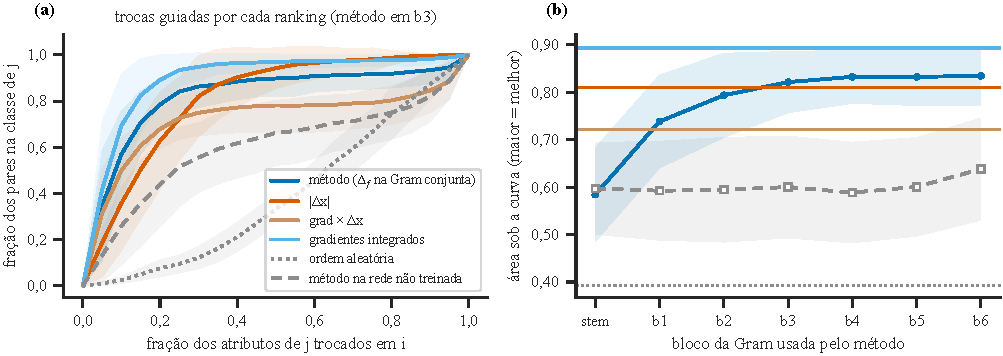
\includegraphics[width=\textwidth]{res_diferencas.pdf}
    \caption{Diferenças entre amostras nas dez bases tabulares. (a) Fração dos pares em que a amostra $i$ passa a ser classificada como $j$ conforme os $k$ primeiros atributos de cada ranking são trocados. (b) Área sob essa curva em função do bloco cuja Gram conjunta define o ranking, com as referências e o piso da rede não treinada.}
    \label{fig:res_diferencas}
\end{figure}

\subsubsection*{Estudos de caso: o método, o SHAP, o LIME, os gradientes integrados e o DiCE}

Na \texttt{letter}, o perceptron atinge acurácia de $0{,}974 \pm 0{,}002$, e cada amostra difere do seu contrafactual, em média, em $9{,}3$ dos 16 atributos. Na \texttt{pendigits}, a acurácia é de $0{,}993 \pm 0{,}002$, e as amostras diferem em $13{,}3$ atributos. A Tabela \ref{tab:res_letter} e as Figuras \ref{fig:res_letter} e \ref{fig:res_pendigits} reúnem os resultados sobre quinhentos pares em cada base.

\begin{table}[pos=htbp]
\centering
\caption{Estudos de caso na \texttt{letter} e na \texttt{pendigits} (cinco sementes, cem pares por semente). Teste contrafactual de trocas (área sob a curva) e fração dos pares em que o atributo em que uma árvore de decisão treinada sobre os rótulos separa $i$ de $j$ está entre os três primeiros de cada ranking, nos pares em que a árvore reproduz as duas predições do perceptron (66 e 79 por semente).}
\label{tab:res_letter}
\footnotesize
\setlength{\tabcolsep}{4pt}
\begin{tabular}{l c c c c}
\hline
 & \multicolumn{2}{c}{\texttt{letter}} & \multicolumn{2}{c}{\texttt{pendigits}} \\
Ranking & Trocas & Árvore, 3 primeiros & Trocas & Árvore, 3 primeiros \\
\hline
Shapley exato com $j$ de referência & $0{,}864$ & $0{,}726$ & $0{,}841$ & $0{,}811$ \\
Gradientes integrados de $x_i$ a $x_j$ & $0{,}860$ & $0{,}711$ & $0{,}839$ & $0{,}808$ \\
\textbf{Método} (Gram conjunta, \texttt{b3}) & $\mathbf{0{,}801}$ & $\mathbf{0{,}705}$ & $\mathbf{0{,}798}$ & $\mathbf{0{,}752}$ \\
LIME contrastivo, margem $f_{c_j} - f_{c_i}$ & $0{,}777$ & $0{,}711$ & $0{,}793$ & $0{,}761$ \\
SHAP, $\phi(x_j) - \phi(x_i)$ & $0{,}776$ & $0{,}629$ & $0{,}774$ & $0{,}714$ \\
$|\Delta x|$ & $0{,}763$ & $0{,}582$ & $0{,}777$ & $0{,}719$ \\
$\nabla f \cdot \Delta x$ & $0{,}703$ & --- & $0{,}711$ & --- \\
SHAP só da amostra $i$ & $0{,}645$ & $0{,}488$ & $0{,}566$ & $0{,}503$ \\
DiCE, frequência de alteração & $0{,}583$ & $0{,}409$ & $0{,}524$ & $0{,}424$ \\
LIME só da amostra $i$ & $0{,}561$ & $0{,}397$ & $0{,}478$ & $0{,}440$ \\
Método na rede não treinada & $0{,}659$ & --- & $0{,}658$ & --- \\
Aleatória entre os que diferem & $0{,}656$ & $0{,}355$ & $0{,}463$ & $0{,}228$ \\
\hline
\end{tabular}
\end{table}

\begin{figure}[pos=htbp]
    \centering
    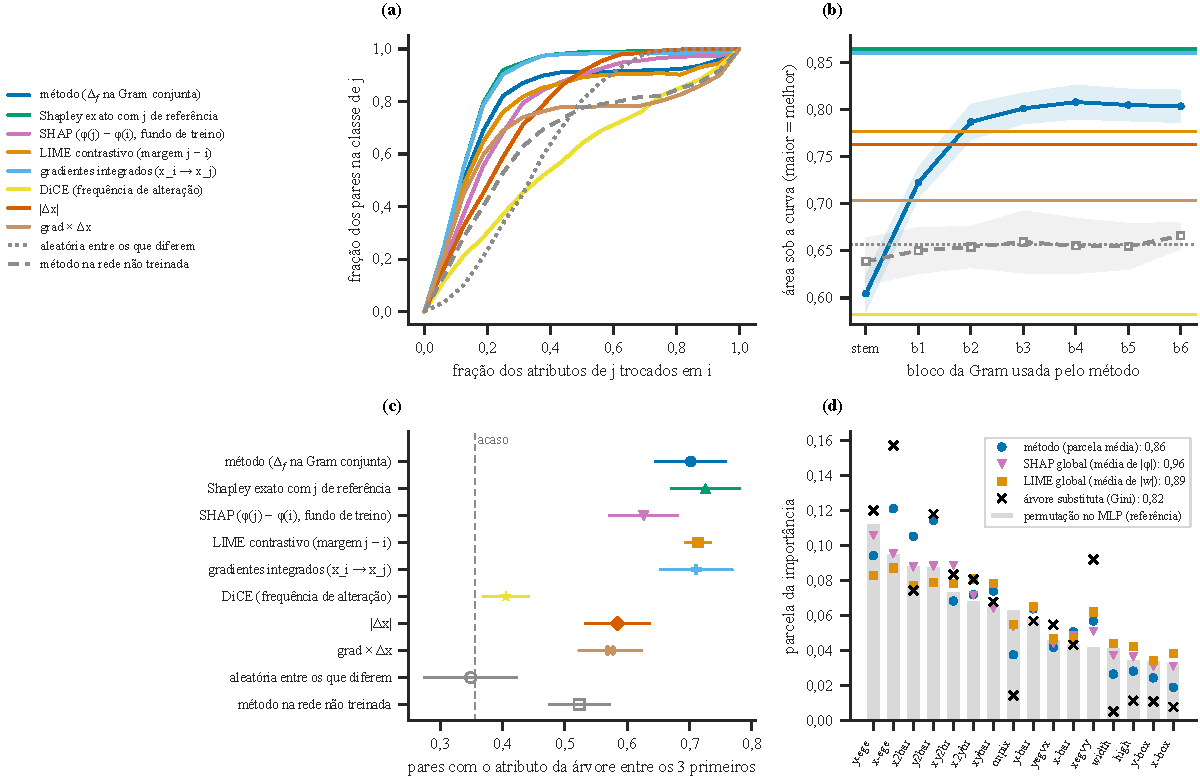
\includegraphics[width=\textwidth]{res_letter.pdf}
    \caption{Estudo de caso na \texttt{letter}. (a) Curvas de trocas de cada ranking, com o método em \texttt{b3}. (b) Área sob a curva do método em função do bloco, com as referências como linhas horizontais (mesmas cores e estilos de (a)). (c) Fração dos pares em que o atributo de separação da árvore de decisão está entre os três primeiros de cada ranking. (d) Importância global normalizada de cada atributo, na ordem da importância por permutação no perceptron (barras), e, na legenda, a correlação de Spearman de cada fonte com ela.}
    \label{fig:res_letter}
\end{figure}

\begin{figure}[pos=htbp]
    \centering
    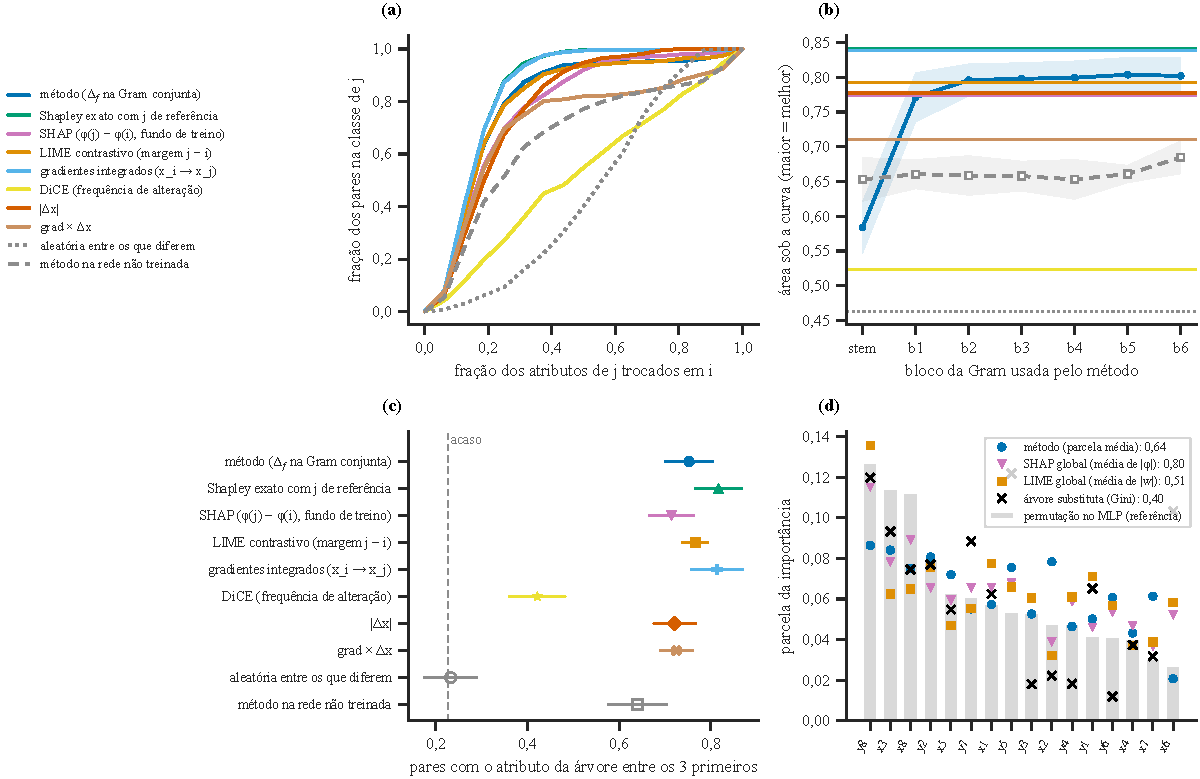
\includegraphics[width=\textwidth]{res_pendigits.pdf}
    \caption{O mesmo estudo de caso da Figura \ref{fig:res_letter} na \texttt{pendigits}, cujos atributos são as coordenadas $(x, y)$ de oito pontos reamostrados ao longo do traço da caneta.}
    \label{fig:res_pendigits}
\end{figure}

O resultado é o mesmo nas duas bases, apesar de os domínios serem distintos. O método supera o SHAP contrastivo em todas as sementes e o LIME contrastivo em três das cinco, e supera com folga as formas usuais, que explicam apenas a amostra $i$ ($0{,}645$ e $0{,}561$ na \texttt{letter}, este último abaixo até da ordem aleatória). A queda é instrutiva: as formas usuais explicam $i$ em relação a uma referência genérica, uma média do treino no SHAP e uma vizinhança amostrada no LIME, e não em relação ao contrafactual $j$, e uma explicação que não é contrastiva não responde à pergunta contrastiva. O método, entretanto, perde nas duas bases para o valor de Shapley exato com $j$ de referência e para os gradientes integrados de $x_i$ a $x_j$, que ficam praticamente empatados entre si. Isso é esperado: ambos são decomposições exatas da variação da margem $f_{c_j} - f_{c_i}$ entre as duas amostras, o primeiro por coalizões e o segundo pelo caminho reto, e o teste de trocas mede justamente essa variação \citep{SundararajanNajmi2020}. O DiCE, por sua vez, fica perto do acaso, porque gera um contrafactual qualquer para a classe de $j$, e não o que distingue $i$ de $j$. A sua pontuação também é a mais custosa, cerca de 26 segundos por par, contra 8 milissegundos do método. O método e o Shapley exato concordam bastante, com correlação de Spearman mediana de $0{,}81$ na \texttt{letter} e $0{,}84$ na \texttt{pendigits} e o mesmo atributo principal em 75\% e 80\% dos pares.

\begin{figure}[pos=htbp]
    \centering
    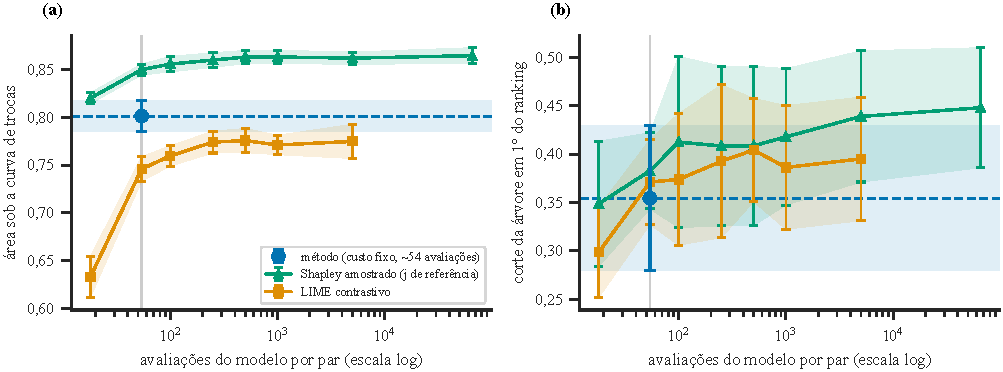
\includegraphics[width=\textwidth]{res_orcamento.pdf}
    \caption{Comparação com o mesmo orçamento de avaliações do modelo por par, na \texttt{letter} (cinco sementes, cem pares por semente). (a) Área sob a curva de trocas. (b) Fração dos pares em que o atributo de separação da árvore de decisão é o primeiro do ranking. As curvas são o valor de Shapley com $j$ de referência, estimado por permutações amostradas (o último ponto é o valor exato, com $2^{16}$ avaliações), e o LIME contrastivo. O método, que tem custo fixo, é o ponto sobre a linha vertical (cerca de 54 avaliações diretas) e a faixa horizontal. Pontos, barras e faixas indicam a média e o desvio padrão entre as sementes.}
    \label{fig:res_orcamento}
\end{figure}

Uma comparação justa precisa considerar o custo. O método não amostra: ele sempre avalia as $F + 2 = 18$ linhas do par, o que equivale a cerca de 54 avaliações diretas do modelo, enquanto o SHAP e o LIME melhoram com mais avaliações. A Figura \ref{fig:res_orcamento} compara as técnicas com o mesmo orçamento. O LIME contrastivo não alcança o método em nenhum orçamento, obtendo $0{,}746$ com as mesmas 54 avaliações e no máximo $0{,}776$. O valor de Shapley com $j$ de referência, ao contrário, supera o método com o mesmo custo, obtendo $0{,}850$, porque uma permutação desse jogo é, literalmente, levar os atributos de $i$ ao valor do contrafactual em uma ordem aleatória e registrar a variação da margem, isto é, o próprio teste. Na corroboração pela árvore, as duas técnicas ficam próximas com o mesmo custo (Figura \ref{fig:res_orcamento}b).

O teste de trocas favorece por construção o Shapley com $j$ de referência e os gradientes integrados, e a árvore é só uma corroboração. A verdade de base sintética resolve essa circularidade (Figura \ref{fig:res_ablacoes}d). Com quatro atributos informativos entre dezesseis e um perceptron com acurácia de $0{,}931$, a fração dos quatro primeiros atributos de cada ranking que são de fato informativos é de $0{,}70$ no Shapley exato, $0{,}65$ nos gradientes integrados, $0{,}60$ no LIME contrastivo e no método, $0{,}49$ no DiCE e em $\nabla f\cdot\Delta x$ e $0{,}33$ na diferença bruta, contra $0{,}25$ do acaso e $0{,}32$ do método na rede não treinada. A ordenação é, portanto, a mesma do teste de trocas: o método identifica os atributos que importam para o rótulo bem acima do acaso e do piso, no nível do LIME, mas abaixo das duas decomposições exatas da margem.

Por fim, o método mostra em que profundidade da rede cada atributo passa a importar, algo que o SHAP e o LIME não separam, e no nível global a sua parcela média concorda com a importância por permutação no perceptron (Spearman de $0{,}86$ na \texttt{letter} e $0{,}64$ na \texttt{pendigits}), menos do que o SHAP ($0{,}96$ e $0{,}80$) (Figuras \ref{fig:res_letter}d e \ref{fig:res_pendigits}d).

\subsubsection*{Nas imagens}

Nas imagens, a leitura usa a Gram cruzada de duas imagens. Sobre vinte pares do Pet, entre raças que o modelo confunde ou da mesma raça com uma classificação correta e outra errada, a deleção ordenada pelo mapa do método reduz a margem $f_{c_i} - f_{c_j}$ mais do que a rede não treinada e a ordem aleatória, com diferenças de área de $0{,}39$ a $0{,}59$ de \texttt{b2} a \texttt{b6}, mas o mapa não se distingue do mapa de centro nesse critério e falha no piso de especificidade: o mesmo mapa calculado contra uma terceira imagem, de raça não envolvida, reduz a margem tanto quanto. A deleção ordenada pelo Grad-CAM contrastivo, calculado sobre o gradiente da mesma margem, produz redução maior da margem a partir de \texttt{b4}. O mapa do Fannar, portanto, não identifica de forma específica as regiões que distinguem a amostra $i$ do contrafactual $j$.

\subsection{P7: As leituras dependem do modelo?}\label{subsec:res_arquitetura}

Esta pergunta é respondida em dois níveis: o mesmo código aplicado a um transformador de visão e o método aplicado a um modelo que não é uma rede neural, a árvore de decisão.

\subsubsection*{O transformador de visão}

\begin{table}[pos=htbp]
\centering
\caption{Leituras por imagem nas três redes de imagem (oito sementes cada, alvo fixo), do \texttt{stem} a \texttt{b6}, e o piso cruzado de cada uma.}
\label{tab:res_arquitetura}
\footnotesize
\setlength{\tabcolsep}{3pt}
\begin{tabular}{l c c c c c c}
\hline
 & \multicolumn{2}{c}{Pet, ResNet} & \multicolumn{2}{c}{Pet, transformador} & \multicolumn{2}{c}{CIFAR-100, ResNet} \\
Leitura & Conjunta & Piso & Conjunta & Piso & Conjunta & Piso \\
\hline
$k$-vizinhos contra a predição & $0{,}095 \to 0{,}619$ & $0{,}07$ & $0{,}146 \to 0{,}571$ & $0{,}05$ & $0{,}060 \to 0{,}701$ & $0{,}07$ \\
AUC da margem para o acerto & $0{,}570 \to 0{,}829$ & $0{,}54$ & $0{,}596 \to 0{,}705$ & $0{,}49$ & $0{,}563 \to 0{,}804$ & $0{,}53$ \\
Confusão suave (Spearman) & $0{,}150 \to 0{,}662$ & $0{,}21$ & $0{,}473 \to 0{,}724$ & $0{,}09$ & $0{,}260 \to 0{,}670$ & $0{,}24$ \\
Contenção em $V_r$ ($r = Q-1$) & $0{,}112 \to 0{,}325$ & $0{,}10$ & $0{,}137 \to 0{,}246$ & $0{,}10$ & $0{,}127 \to 0{,}358$ & $0{,}13$ \\
$\widehat{E}_{\mathrm{ratio}}$ para o erro & $0{,}498 \to 0{,}641$ & $0{,}54$ & $0{,}525 \to 0{,}649$ & $0{,}53$ & $0{,}469 \to 0{,}672$ & $0{,}53$ \\
Hierarquia semântica (P9) & $0{,}514 \to 0{,}693$ & $0{,}64$ & $0{,}605 \to 0{,}669$ & $0{,}61$ & $0{,}638 \to 0{,}849$ & $0{,}66$ \\
\hline
\end{tabular}
\end{table}

As leituras por imagem se transferem ao transformador sem nenhuma alteração do código (Tabela \ref{tab:res_arquitetura}): todas superam o piso em todas as sementes a partir de \texttt{b2}, inclusive a razão de energia ortogonal, que falha nos blocos rasos das ResNets. O que muda é a origem da informação. No transformador, o gradiente contrastivo isolado quase não carrega informação sobre o comportamento (o seu $k$-vizinhos fica em torno de $0{,}11$ em todos os blocos), e a composição só supera as ativações de forma consistente no \texttt{stem}, de modo que a decomposição contra a CKA favorece a CKA a partir de \texttt{b2}. A contenção em $V_r$, por outro lado, continua favorecendo a composição em todos os blocos. Sendo assim, a forma do método independe da arquitetura, mas a contribuição de cada fonte não: o que o gradiente acrescenta às ativações é uma propriedade da rede convolucional, e não do método.

\begin{figure}[pos=htbp]
    \centering
    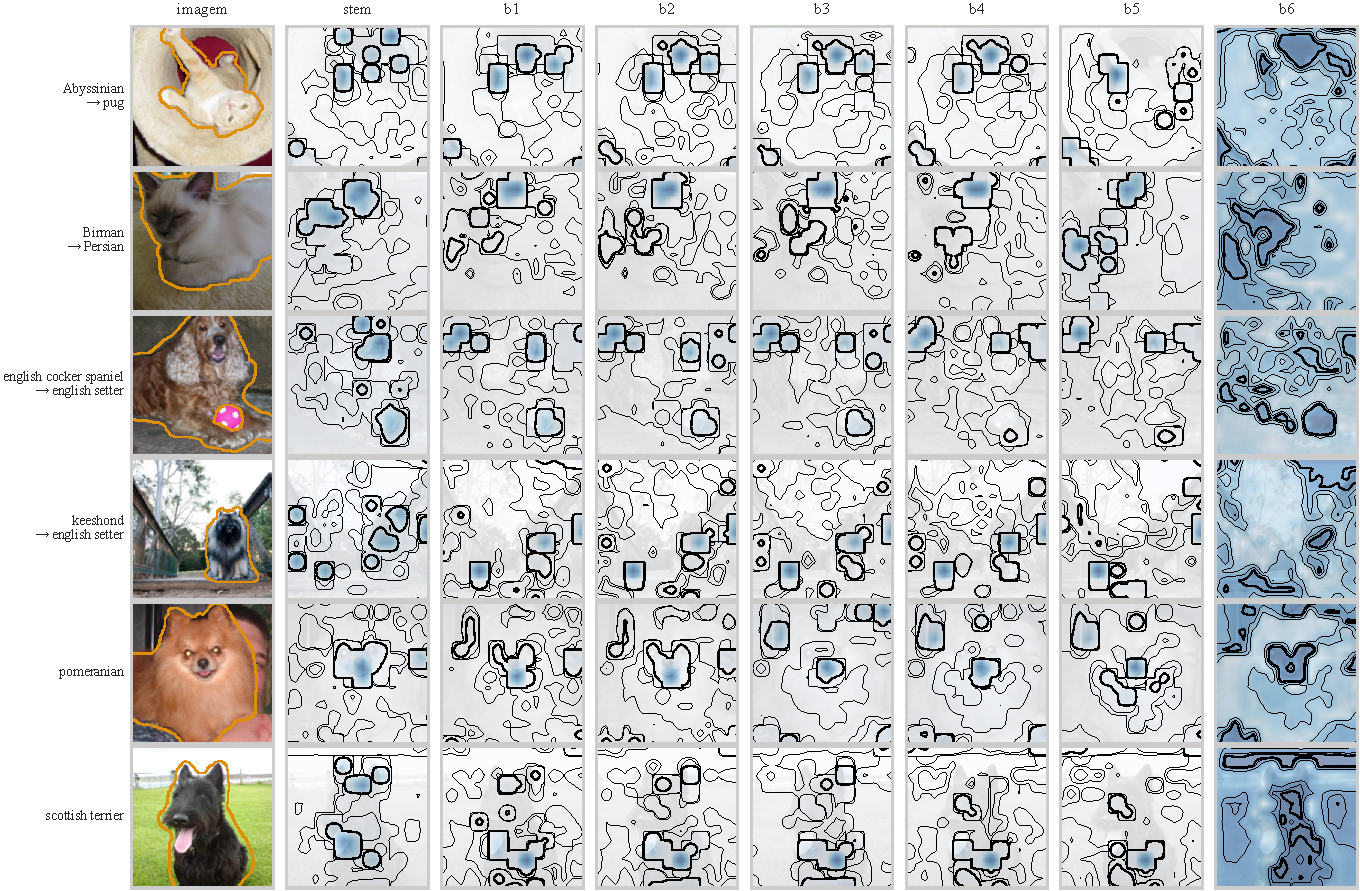
\includegraphics[width=\textwidth]{res_campo_vit.pdf}
    \caption{Campo de energia da Gram conjunta do transformador sobre as mesmas imagens da Figura \ref{fig:res_campo_resnet}. O aspecto quadriculado vem da grade de \textit{tokens} ($16 \times 16$), ampliada para a imagem. No último bloco, a cabeça é um \textit{pooling} médio seguido de uma camada linear, de modo que o gradiente é o mesmo em todas as posições e o campo deixa de distinguir regiões.}
    \label{fig:res_campo_vit}
\end{figure}

As leituras sobre a entrada, entretanto, não se transferem. No transformador, a fração da energia sobre o animal cai de $0{,}84$ no \texttt{stem} para $0{,}60$ a $0{,}67$ nos blocos seguintes, no nível do mapa de centro ($0{,}66$) ou abaixo dele, e para $0{,}51$ no último bloco, e o teste de deleção fica abaixo do centro em todos os blocos após o \texttt{stem} (Figura \ref{fig:res_campo_vit}). A explicação mais provável é estrutural: a atenção mistura informação de toda a imagem já nas primeiras camadas \citep{Raghu2021}, e o vetor de um \textit{token} deixa de descrever apenas a sua posição. Por esse motivo, as leituras espaciais em transformadores costumam propagar a relevância através da atenção \citep{Chefer2021}. Essa explicação, contudo, não foi separada da baixa acurácia do modelo ($0{,}438 \pm 0{,}011$).

\subsubsection*{O método aplicado a uma árvore de decisão}

O segundo nível testa se o método é, de fato, modelo-agnóstico. Uma árvore de decisão é treinada sobre os rótulos da \texttt{letter} e da \texttt{pendigits} e analisada com as fontes de caminho, folga e classes, com a mesma composição e a mesma leitura de pares utilizadas nas redes, e as suas leituras são comparadas com uma resposta conhecida, a explicação que a própria árvore fornece pelo seu caminho de decisão.

A Figura \ref{fig:res_arvore_caminhos} mostra, para dois pares da \texttt{letter}, essa explicação e a leitura do método lado a lado. O método não tem acesso à regra de decisão da árvore: ele apenas compõe as três fontes e mede quanto levar cada atributo ao valor do contrafactual aproxima $i$ de $j$. Ainda assim, o atributo testado no nó de separação passa a responder por praticamente toda a pontuação exatamente na profundidade em que os caminhos se separam. Nas profundidades anteriores, os dois caminhos são idênticos, e a única fonte que distingue as amostras é a folga, isto é, o quanto cada uma está distante dos limiares que ambas atravessaram.

\begin{figure}[pos=htbp]
    \centering
    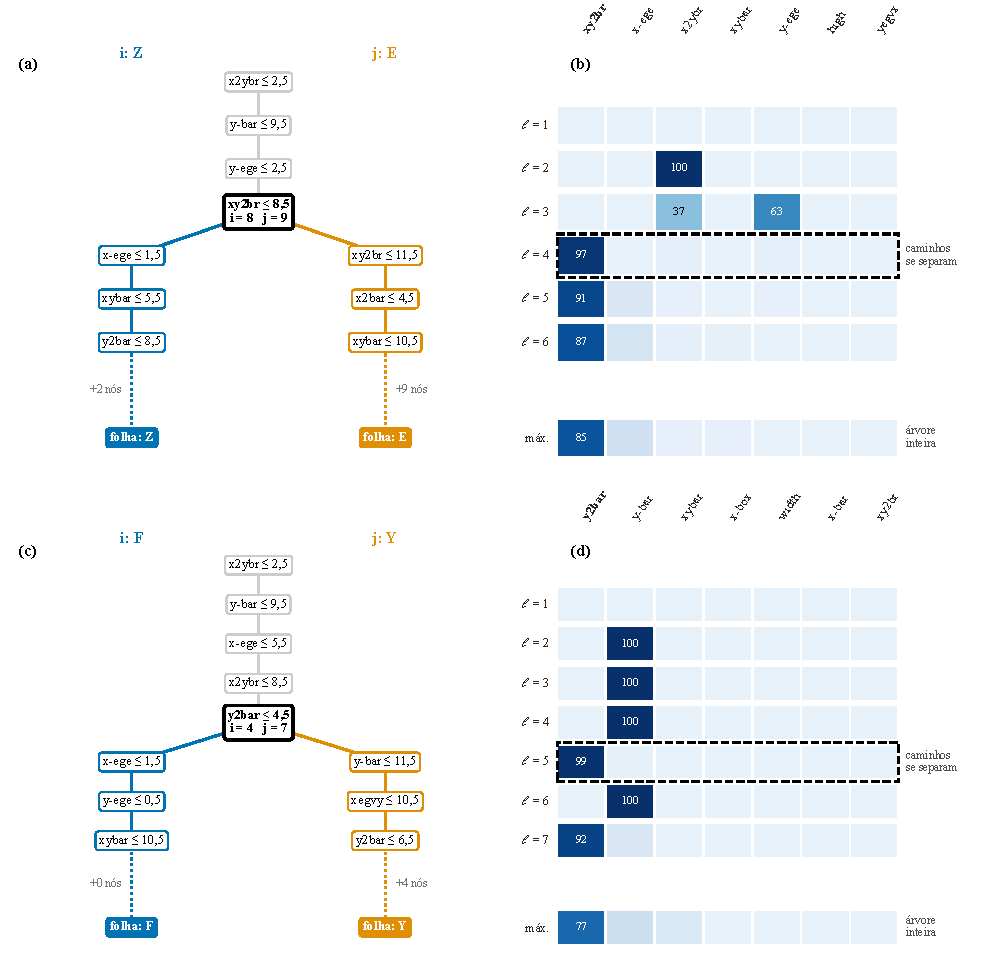
\includegraphics[width=\textwidth]{res_arvore_caminhos.pdf}
    \caption{A explicação da árvore de decisão e a leitura do método, lado a lado, para dois pares da \texttt{letter} (semente 0). (a, c) Caminhos das amostras $i$ e $j$ na árvore: o trecho comum, o nó de separação (destacado, com os valores de $i$ e de $j$ no atributo testado) e os ramos até as folhas, com os nós intermediários omitidos. (b, d) Parcela de cada atributo, em porcentagem, na pontuação $\Delta_f$ do método em cada profundidade $\ell$, alinhada verticalmente com a árvore. A linha tracejada marca a profundidade em que os caminhos se separam, e a última linha é a árvore inteira. As colunas são os atributos que diferem entre $i$ e $j$, na ordem do ranking final do método, e o atributo de separação está em negrito. Os dois pares ilustram o caso típico, em que a datação do método coincide com a da árvore (79\% dos pares).}
    \label{fig:res_arvore_caminhos}
\end{figure}

\begin{table}[pos=htbp]
\centering
\caption{O método aplicado a uma árvore de decisão (cinco sementes, cem pares por semente). Fração dos pares em que o atributo do nó em que os caminhos de $i$ e $j$ se separam é o primeiro de cada ranking, e área sob a curva do teste de trocas feito na própria árvore.}
\label{tab:res_arvore}
\footnotesize
\setlength{\tabcolsep}{4pt}
\begin{tabular}{l c c c c}
\hline
 & \multicolumn{2}{c}{\texttt{letter}} & \multicolumn{2}{c}{\texttt{pendigits}} \\
Ranking & Corte em 1º & Trocas & Corte em 1º & Trocas \\
\hline
\textbf{Método} (caminho $\circ$ folga $\circ$ classes) & $\mathbf{0{,}850}$ & $\mathbf{0{,}658}$ & $\mathbf{0{,}908}$ & $\mathbf{0{,}692}$ \\
Método sem a fonte de caminho (folga $\circ$ classes) & $0{,}762$ & $0{,}641$ & $0{,}846$ & $0{,}693$ \\
Só caminho & $0{,}976$ & $0{,}630$ & $0{,}998$ & $0{,}672$ \\
Só folga & $0{,}824$ & $0{,}619$ & $0{,}918$ & $0{,}691$ \\
Só classes & $0{,}472$ & $0{,}598$ & $0{,}490$ & $0{,}600$ \\
Shapley exato com $j$ de referência & $0{,}760$ & $0{,}892$ & $0{,}736$ & $0{,}923$ \\
$|\Delta x|$ & $0{,}240$ & $0{,}713$ & $0{,}302$ & $0{,}730$ \\
Aleatória entre os que diferem & $0{,}132$ & $0{,}655$ & $0{,}074$ & $0{,}512$ \\
Método na árvore de rótulos embaralhados & $0{,}158$ & $0{,}497$ & $0{,}114$ & $0{,}426$ \\
\hline
\end{tabular}
\end{table}

\begin{figure}[pos=htbp]
    \centering
    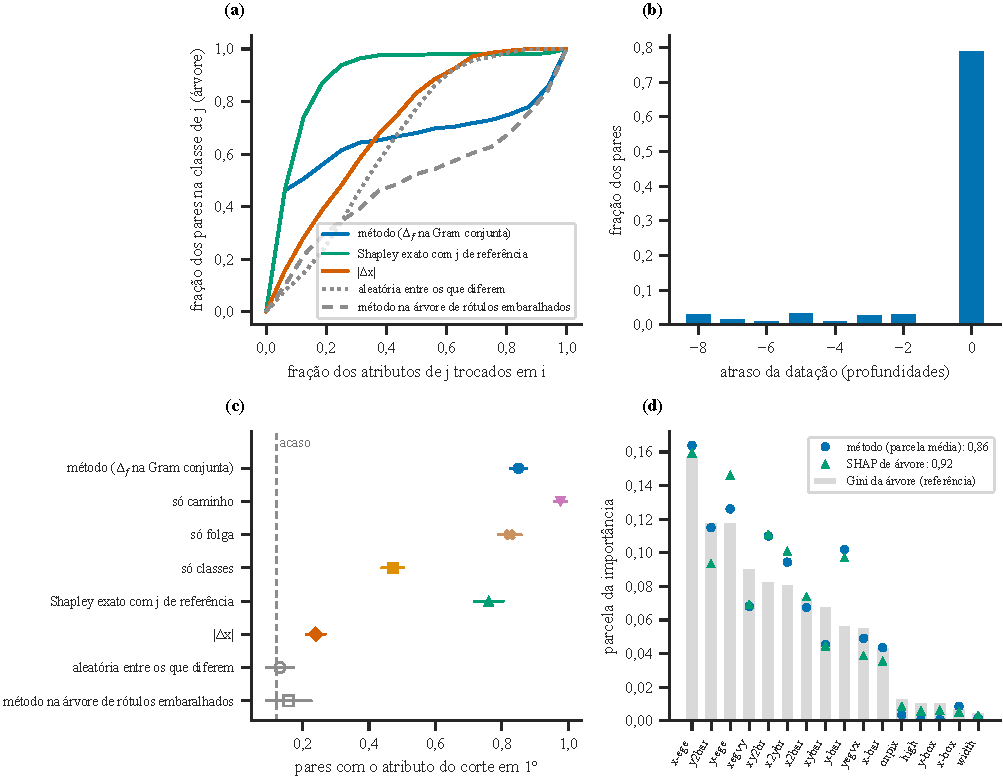
\includegraphics[width=\textwidth]{res_arvore.pdf}
    \caption{O método aplicado a uma árvore de decisão na \texttt{letter}. (a) Teste de trocas na própria árvore. (b) Diferença entre a profundidade em que o atributo de separação passa a ser o primeiro do método e a profundidade em que os caminhos de $i$ e $j$ se separam. (c) Fração dos pares em que o atributo de separação é o primeiro de cada ranking. (d) Importância global normalizada, na ordem da importância de Gini da árvore. Na legenda, a correlação de Spearman de cada fonte com ela.}
    \label{fig:res_arvore}
\end{figure}

Em termos agregados (Tabela \ref{tab:res_arvore}), o atributo do nó de separação é o primeiro do método em 85\% dos pares na \texttt{letter} e em 91\% na \texttt{pendigits}, contra 76\% e 74\% do Shapley exato, 24\% e 30\% da diferença bruta e 16\% e 11\% do piso. A fonte de caminho sozinha alcança 98\% e 100\%, o que é quase uma consequência da construção, visto que trocar esse atributo é o que muda o caminho de $i$, e a fonte de folga também é definida sobre os nós atravessados. Por isso o estudo foi repetido sem a fonte de caminho: a recuperação cai para 76\% e 85\%, ainda no nível do Shapley exato na \texttt{letter} e acima dele na \texttt{pendigits}, de modo que ela não depende da fonte que já codifica o nó de separação. O resultado mais forte é a datação: a profundidade em que o atributo de separação passa a ser o primeiro do método coincide com a profundidade da separação em 79\% dos pares na \texttt{letter} e em 86\% na \texttt{pendigits}, nunca ocorre depois dela e não se altera sem a fonte de caminho (Figura \ref{fig:res_arvore}b). Nos demais pares, ela ocorre antes, quase sempre porque um nó acima da separação testa o mesmo atributo e a folga registra essa proximidade de um limiar. No nível global, a parcela média do método tem correlação de $0{,}86$ e $0{,}71$ com a importância de Gini e de $0{,}89$ e $0{,}74$ com o SHAP de árvore \citep{Lundberg2020}.

O mesmo experimento expõe o principal limite da leitura de pares. No teste de trocas na própria árvore, o método obtém $0{,}658$ e $0{,}692$, abaixo da diferença bruta ($0{,}713$ e $0{,}730$), e precisa, em média, de $5{,}5$ e $5{,}0$ trocas para produzir um contrafactual válido, contra $1{,}8$ e $1{,}6$ do contrafactual mínimo, obtido por enumeração. A causa é que $\Delta_f$ troca um atributo de cada vez: os atributos que só importam depois que $i$ atravessa o corte não alteram nada quando trocados sozinhos, e ficam em ordem arbitrária no ranking. O valor de Shapley, que considera todas as combinações de trocas, enxerga essas interações. Sendo assim, a leitura de pares responde o que distingue $i$ do seu contrafactual, e não o menor conjunto de mudanças que basta para que $i$ se torne $j$.

\subsection{P8: Em que profundidade a decisão se forma?}\label{subsec:res_datacao}

A intervenção da Equação \eqref{eq:intervencao} fornece uma datação externa ao método: depois que a decisão está formada, o estado passa a ser redundante com ela e se torna robusto a perturbações. A correlação de Spearman entre essa estabilidade e a recuperação da decisão pela Gram conjunta é de $0{,}64 \pm 0{,}28$ nas bases tabulares, $0{,}89 \pm 0{,}05$ na ResNet do Pet, $1{,}00$ no transformador e $0{,}75 \pm 0{,}07$ no CIFAR-100.

Essa concordância, entretanto, é inflada pelo fato de as duas séries crescerem com a profundidade. O mesmo problema é conhecido nas sondagens lineares, em que a capacidade de decodificar uma propriedade cresce com a profundidade sem indicar onde o modelo a utiliza \citep{Belinkov2022}. Calculada sobre as diferenças entre blocos consecutivos, que removem essa tendência comum, a concordância cai, mas não desaparece em três das quatro famílias: $0{,}51 \pm 0{,}34$ nas bases tabulares (positiva em 92\% das execuções, $p < 0{,}001$), $0{,}43 \pm 0{,}14$ na ResNet do Pet e $0{,}58 \pm 0{,}30$ no transformador (positiva nas oito sementes, $p = 0{,}008$). No CIFAR-100, ela cai para $0{,}16 \pm 0{,}21$ e não se distingue de zero ($p = 0{,}17$). Isto é, nas bases tabulares e no Pet, os blocos em que a decisão mais se estabiliza são os blocos em que a geometria mais ganha, e não apenas os mais profundos. A verificação mais direta, entretanto, vem da árvore de decisão, em que a profundidade da decisão é conhecida para cada par e o método a acerta exatamente em 79\% e 86\% dos pares, com ou sem a fonte de caminho.

\subsection{P9: As distâncias refletem uma organização semântica que o modelo nunca viu?}\label{subsec:res_semantica}

\begin{figure}[pos=htbp]
    \centering
    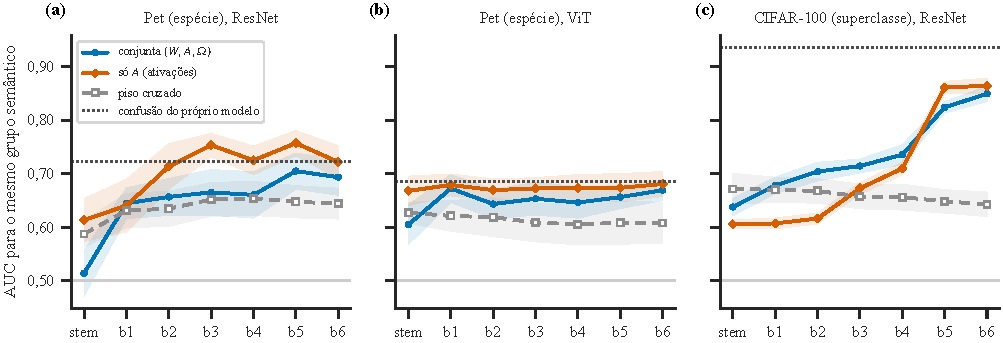
\includegraphics[width=\textwidth]{res_semantica.pdf}
    \caption{Hierarquia semântica externa (alvo fixo, oito sementes). Área sob a curva ROC com que a proximidade média entre duas classes separa os pares de classes do mesmo grupo semântico (a espécie no Pet e a superclasse no CIFAR-100), por bloco, para a Gram conjunta, a fonte de ativações e o piso cruzado. A linha pontilhada é a mesma área calculada sobre a confusão suave do próprio modelo, e a faixa é o desvio entre sementes. (a) ResNet do Pet. (b) Transformador do Pet. (c) ResNet do CIFAR-100.}
    \label{fig:res_semantica}
\end{figure}

A Figura \ref{fig:res_semantica} compara as distâncias entre classes com a hierarquia de cada base, que não entra no treinamento. No CIFAR-100, a área sob a curva cresce de $0{,}64$ no \texttt{stem} para $0{,}85$ em \texttt{b6}, contra um piso que cai de $0{,}67$ para $0{,}64$, e supera o piso em todas as sementes a partir de \texttt{b3}: classes da mesma superclasse ficam, de fato, mais próximas no espaço construído. A composição supera as ativações do \texttt{stem} a \texttt{b4} em todas as sementes, e as ativações a superam nos dois últimos blocos. No Pet, a leitura também supera o piso, mas de forma menos consistente: na ResNet, em todas as sementes apenas no último bloco ($0{,}69$ contra $0{,}64$), e no transformador, na maioria das sementes ($0{,}64$ a $0{,}67$ contra $0{,}61$). O piso é alto porque cor e textura já se correlacionam com a espécie, e as ativações isoladas superam a composição em quase todos os blocos.

A comparação decisiva é com o comportamento. A mesma área calculada sobre a confusão suave do modelo é de $0{,}94$ no CIFAR-100, $0{,}72$ na ResNet do Pet e $0{,}68$ no transformador, isto é, maior do que a da Gram conjunta em todos os blocos. Só as ativações isoladas da ResNet do Pet chegam a superá-la, por pouco. O modelo já confunde mais as classes semanticamente próximas, e a geometria reflete essa organização sem ir além dela. A resposta a P9 é, portanto, afirmativa no sentido de que as distâncias carregam uma hierarquia semântica que o modelo nunca viu, mas essa hierarquia é a que o próprio comportamento do modelo já expressa, e não uma informação semântica adicional.

\subsection{Custo computacional medido}\label{subsec:res_custo}

A análise da Subseção \ref{subsec:custo} foi verificada medindo o tempo de cada etapa enquanto o tamanho do problema cresce. Em escala logarítmica, um custo $\Theta(n^a)$ aparece como uma reta de inclinação $a$, e é essa inclinação que a Figura \ref{fig:res_complexidade} reporta.

\begin{figure}[pos=htbp]
    \centering
    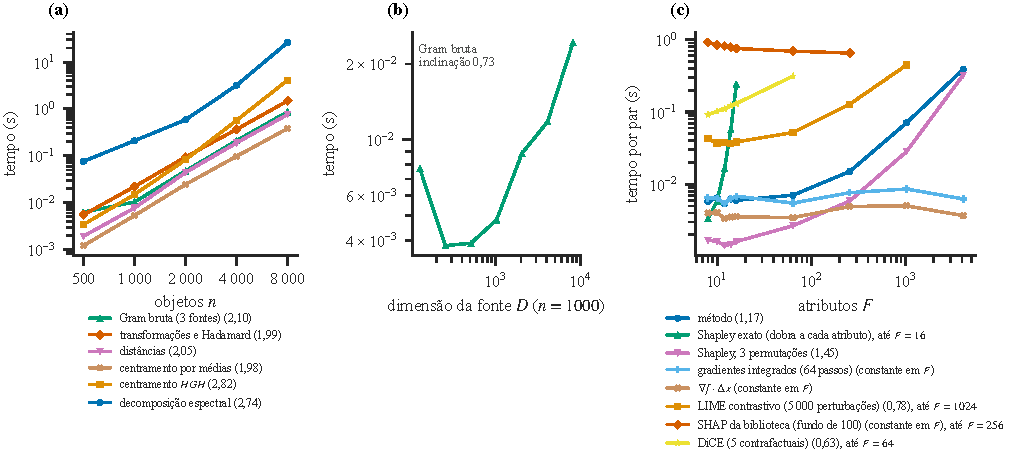
\includegraphics[width=\textwidth]{res_complexidade.pdf}
    \caption{Tempo das etapas do método em função do tamanho do problema, em escala logarítmica nos dois eixos. Entre parênteses está a inclinação ajustada nos três maiores tamanhos, que estima o expoente do custo. (a) Etapas da construção e das leituras em função do número de objetos $n$, com três fontes de dimensão 256. (b) Matriz de Gram bruta em função da dimensão $D$ da fonte, com $n = 1\,000$. (c) Tempo por par da leitura de diferenças em função do número de atributos $F$, comparado ao de todas as técnicas de P6, com as configurações dos estudos de caso: o valor de Shapley exato com $j$ de referência, a sua estimativa por três permutações, os gradientes integrados, $\nabla f\cdot\Delta x$, o LIME contrastivo, o SHAP da biblioteca e o DiCE. As técnicas cujo custo não depende de $F$ estão marcadas como constantes, e as mais caras foram medidas até o $F$ indicado. Todas as medidas são em CPU, num perceptron multicamadas residual de largura 256.}
    \label{fig:res_complexidade}
\end{figure}

Os expoentes medidos são compatíveis com os previstos. A matriz de Gram bruta cresce com expoente $2{,}10$ em $n$. Em $D$, a inclinação ($0{,}73$) fica abaixo de 1 porque, nas dimensões pequenas, o custo fixo das rotinas de álgebra linear ainda pesa, e o tempo só passa a crescer de forma aproximadamente linear a partir de $D = 1\,024$. As transformações, a matriz de distâncias e a seleção dos vizinhos crescem com expoente próximo de 2, e a decomposição espectral com $2{,}74$. As alternativas quadráticas da Tabela \ref{tab:custo} também se confirmam: o centramento pelas médias de linhas e colunas leva $0{,}38$ s com $n = 8\,000$, contra $4{,}1$ s do produto $H\widetilde{\mathbf{G}}H$. Com $n \approx 500$, entretanto, a decomposição leva cerca de $76$ ms, e o custo total é dominado pela extração das fontes.

A Figura \ref{fig:res_complexidade}c compara o custo por par da leitura de diferenças com o de todas as técnicas de P6, e as técnicas se separam em quatro grupos. O primeiro é o valor de Shapley exato, cujo tempo dobra a cada atributo acrescentado: de $3$ ms com $F = 8$ para $241$ ms com $F = 16$, de modo que, com algumas dezenas de atributos, ele deixa de ser viável. O segundo reúne as técnicas lineares em $F$: o método, que avalia $F + 2$ linhas numa passagem direta e numa reversa (expoente $1{,}17$, com $6$ ms em $F = 16$ e $0{,}39$ s em $F = 4\,096$), e o Shapley estimado por três permutações, que avalia $3(F+1)$ linhas apenas com passagens diretas e é, por isso, de duas a quatro vezes mais rápido até $F = 1\,024$, com os dois próximos em $F = 4\,096$ ($0{,}39$ e $0{,}32$ s). O terceiro é o das técnicas de custo constante em $F$, os gradientes integrados (64 passagens, cerca de $6$ ms) e $\nabla f\cdot\Delta x$ (uma passagem, cerca de $4$ ms), cujo número de avaliações não depende do número de atributos. O quarto é o das técnicas por amostragem, que são as mais caras em toda a faixa medida: o LIME contrastivo, com $5\,000$ perturbações e uma regressão ponderada, leva de $40$ ms a $0{,}45$ s (expoente $0{,}78$); o SHAP da biblioteca, com um fundo de 100 amostras, leva de $0{,}65$ a $0{,}92$ s, praticamente constante enquanto o orçamento mínimo de avaliações não é atingido; e o DiCE leva de $0{,}09$ a $0{,}31$ s até $F = 64$, com chamadas isoladas que, quando a busca aleatória demora a encontrar um contrafactual, chegam a dezenas de segundos. O método é, portanto, exponencialmente mais barato que o Shapley exato, cerca de seis vezes mais barato que o LIME contrastivo e de vinte a cem vezes mais barato que o DiCE e o SHAP da biblioteca, e da mesma ordem que o Shapley por permutações, e só é mais caro do que as atribuições por gradiente, que, por outro lado, exigem que o modelo seja diferenciável em relação à entrada.

\subsection{Síntese dos resultados}\label{subsec:res_sintese}

A Tabela \ref{tab:res_sintese} resume a resposta a cada pergunta e a condição em que ela vale. O padrão geral é que a geometria reflete a decisão, o erro e, onde o modelo confunde de forma estruturada, a confusão e a hierarquia semântica, mas não antecipa esse comportamento melhor do que o próprio modelo; que a composição acrescenta o gradiente às ativações nas redes convolucionais, sem que a forma multiplicativa importe; e que, nas leituras locais, o método é competitivo com as técnicas de atribuição usuais, mas perde para as decomposições exatas da margem.

\begin{table}[pos=htbp]
\centering
\caption{Síntese das respostas às perguntas P1 a P9 e das condições em que valem.}
\label{tab:res_sintese}
\footnotesize
\begin{tabular}{p{0.7cm}p{5.4cm}p{7.2cm}}
\hline
 & Resposta & Condição ou limite \\
\hline
P1 & Afirmativa para a decisão e para o erro, acima do piso em todas as bases. & A margem geométrica não supera o \textit{softmax} nem o \textit{trust score}; nos blocos profundos, a Gram iguala as ativações e os \textit{logits}; confusão só quando o modelo confunde de forma estruturada. \\
P2 & Condicionada: a composição supera as ativações nos blocos rasos e intermediários das redes convolucionais. & O ganho vem do gradiente, que isolado iguala a composição na ResNet do Pet; o produto de Hadamard e a soma são equivalentes; $T_a$ é essencial e $\mathbf{J}$ é irrelevante. \\
P3 & Condicionada: o método vê além da CKA onde o gradiente acrescenta às ativações. & Nas bases tabulares e no transformador, o resultado favorece a CKA. \\
P4 & A contenção das direções de classe em $V_r$ é a leitura mais robusta. & $\widehat{E}_{\mathrm{ratio}}$ para o erro só supera o piso nos blocos profundos das redes convolucionais. \\
P5 & Localiza o animal e descreve a organização espacial das representações. & A localização vem principalmente do gradiente; no teste de deleção, o Grad-CAM produz maior queda de margem a partir de \texttt{b4}; não se transfere ao transformador. \\
P6 & Supera SHAP e LIME contrastivos e as formas usuais na \texttt{letter} e na \texttt{pendigits}; identifica atributos informativos bem acima do acaso; aproxima o Shapley exato (Spearman de $0{,}81$ e $0{,}84$) com custo linear, contra exponencial. & Perde para o Shapley exato e para os gradientes integrados em todos os testes; empata com $|\Delta x|$ nas dez bases; nas imagens não passa no piso de especificidade; troca um atributo por vez. \\
P7 & Leituras por imagem se transferem ao transformador; na árvore, o nó de separação é o primeiro em 85\% e 91\% dos pares. & Leituras espaciais não se transferem; sem a fonte de caminho, a recuperação cai para 76\% e 85\%, no nível do Shapley exato. \\
P8 & Concordância com a intervenção sobrevive à remoção da tendência nas bases tabulares e no Pet. & Não sobrevive no CIFAR-100; a verificação mais direta é a árvore (79\% e 86\%). \\
P9 & As distâncias refletem a hierarquia semântica acima do piso nos blocos profundos. & Abaixo da hierarquia já presente na confusão do próprio modelo; no Pet, o piso é alto. \\
\hline
\end{tabular}
\end{table}
